\section{CPU-level Energy Measurements}
\label{sec:energymeasure}

High precision instruction level energy models can be derived for pipelined
processors by monitoring the instantaneous current drawn by the processor at
each clock cycle, as explained in \cite{nikolaidis2005instruction}. Modern
processors commonly operate at a few GHz, and the Nyquist-Shannon sampling theorem
\cite{nyquist1928certain} states that the sampling frequency must be at least
twice the frequency of the signal being measured. The signal sampled from the
processor might change at least once per clock cycle, so obtaining accurate
measurements would require use of very expensive instruments.

\begin{figure}[tbh]
    \centering
    \input{figs/test_setup.tex}
    \caption{Bench setup for measuring single instruction current drain.}
    \label{fig:setup}
\end{figure}

In \cite{rundehvatum2013exploring}, single instructions were measured by
exploting fast-loop-mode and looping over a group of equal instructions. An
Agilent bench multimeter and a shunt resistor were set up like shown in
\autoref{fig:setup}. This method provides an average power consumption when the
pipeline is (mostly) filled with a single type of instruction. Instead of using
a serial connected ammeter, the power rail is connected in series with a shunt
resistor equal to the one seen in \autoref{fig:shunt}, and voltage drop over
this resistor is measured using a voltmeter. This method provides a way to
measure currents either outside the range of the ammeter or with greater
accuracy than using the built-in ammeter. An example of how a shunt resistor can
provide better accuracy; when an Agilent 34410A is used to measure a current in
which the voltage exeeds 0.8~V, the readings is within 0.1~\% when the system is
correctly calibrated. If a shunt resistor with the right characteristics is
used, the voltage drop across the shunt resistor will lie in the range 0 --
100~mV, and then readings will, according to the datasheet, be within 0.003~\%
\cite{agilent34410a}.

\begin{figure}[tbh]
    \centering
    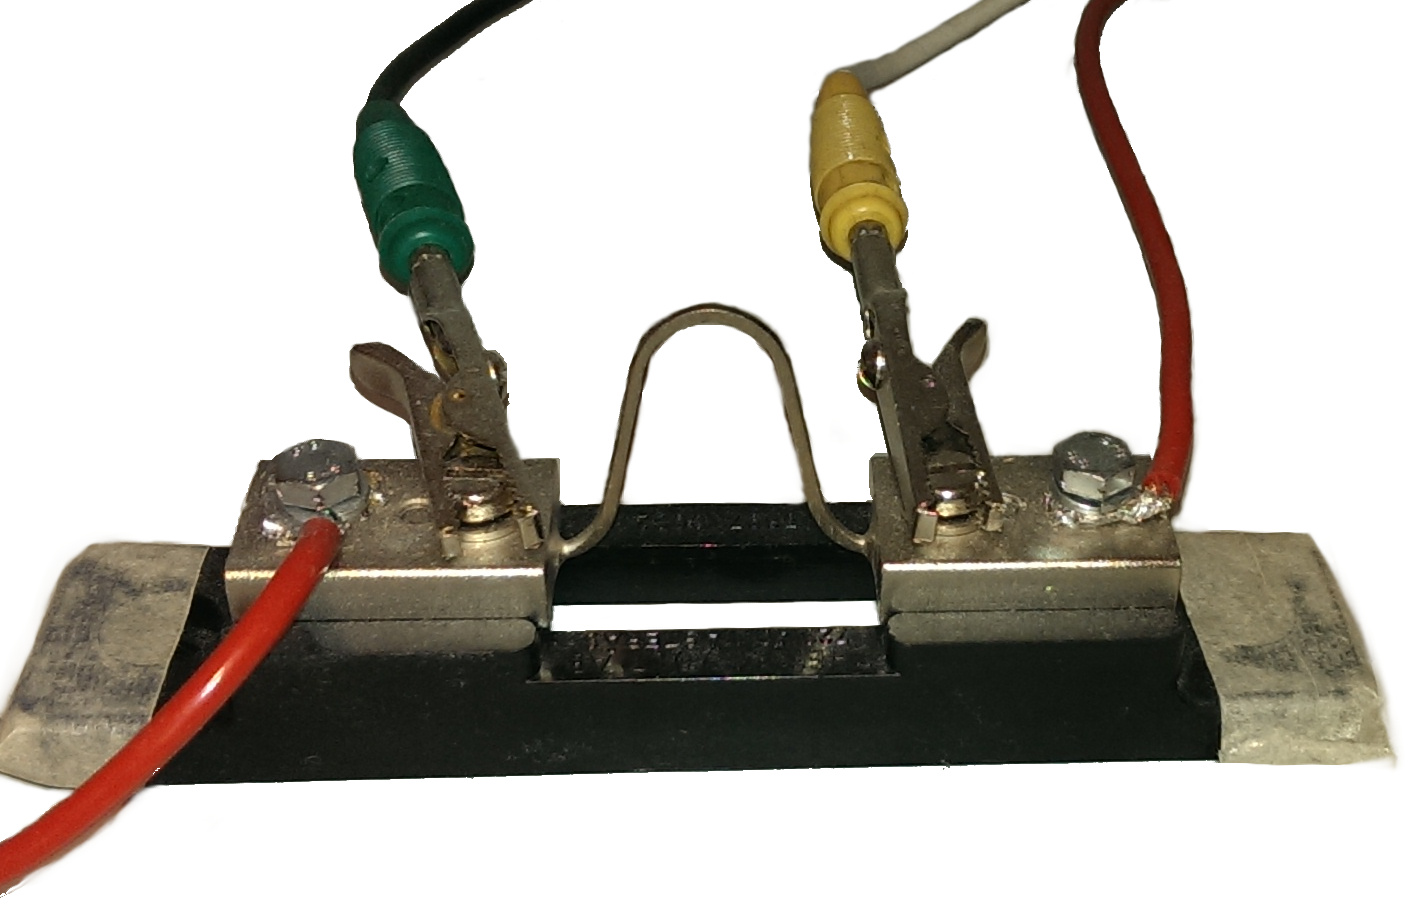
\includegraphics[width=0.8\textwidth]{figs/shunt.jpg}
    \caption{An example shunt resistor.}
    \label{fig:shunt}
\end{figure}

\begin{figure}[tbh]
    \centering
    \input{figs/varcurrent.tex}
    \caption{Current measurement of a variable load.}
    \label{fig:varcurrent}
\end{figure}


